%File: formatting-instruction.tex
\documentclass[letterpaper]{article}
\usepackage{aaai}
\usepackage{times}
\usepackage{helvet}
\usepackage{courier}
\usepackage{todonotes}
\usepackage{amssymb}
\usepackage{amsmath}
\usepackage{hyperref}
%\usepackage{subcaption}

\frenchspacing
\setlength{\pdfpagewidth}{8.5in}
\setlength{\pdfpageheight}{11in}


\pdfinfo{
/Title (Formatting Instructions for Authors Using LaTeX)
/Subject (AAAI Publications)
/Author (anonymous)}
\setcounter{secnumdepth}{0}  

\newcommand{\mytodo}[1]{\textbf{[[#1]]}}


 \begin{document}
% The file aaai.sty is the style file for AAAI Press 
% proceedings, working notes, and technical reports.
%
\title{Interactive Bayesian Optimization for Game Mechanics}
\author{
}
% % AZ: note - technically we don't have the standard notion of ``interaction'' for the GP DDA



\maketitle
\begin{abstract}
\begin{quote}
\mytodo{fill me}
\end{quote}
\end{abstract}

\section{Introduction}

\noindent Game design and development often involves a final phase of substantial fine-tuning of game mechanics. Paradigmatic examples include varying the settings of player character movement parameters, altering opponent combat statistics, or varying low-level parameters around movement and collision of game objects. Tuning is often a time-consuming and expensive process due to the need for human testing (rather than analytic solutions or simulation results) and the large space of possible parameter settings for a game.
%\begin{enumerate}
%\item parameter values must be set to (globally) optimal values, requiring search over a large space
%\item evaluating a set of parameter values cannot be done analytically or via simulation, but requires costly (in terms of time and money) direct human evaluation
%\item quality of a set of parameters may be difficult to specify on a global scale, and depend on other sets of parameters
%\end{enumerate}
%We ask: %can an artificially intelligent system efficiently automate the tuning process? 
%can an artificially intelligent (AI) system act as a designer focused on the problem of parameter tuning?
%Can such a system acquire design knowledge of low-level parameter settings that achieve design goals tailored to individual players?
%In this paper, we ask the following questions. %can an artificially intelligent system efficiently automate the tuning process? 
%Can an artificially intelligent (AI) system learn a model of the {\em design space} of the tunable parameters of the game?
%Can the system apply the design space model to the problem of parameter tuning to assist game developers or tailor game play to individuals?
%Can such a system acquire design knowledge of low-level parameter settings that achieve design goals tailored to individual players?

%%% MOR: probably needs to be rewritten:
Our long term goal is to develop an intelligent system that can learn to model the design of computer games.
To do so will enable the development of practical systems and tools that can:

\begin{itemize}
%\item A critical step toward a theory of the design of game mechanics.
\item Help game developers visualize, understand, and select amongst parameters with complex tradeoffs.
\item Automatically tune the parameters of a game to meet design goals, taking into account a large population of diverse players.
\item Automatically tune the parameters of a game to tailor game play to specific individual players.
\end{itemize}

Our central insight is to formulate the iterative design process as a form of active learning in which game players respond to an AI-chosen sent of tuning parameters.
%with players responding to an AI-chosen game tuning. 
Specifically, an {\em Interactive Bayesian Optimization} model for active learning makes explicit the trade-offs between improving a design and testing alternatives, while developing a model of the design space of a given game for later \mytodo{(re)use}.
%From this perspective, 
%A {\em design space} is a multi-dimensional domain of possible game parameter values that map to expected player behavior (and associated levels of uncertainty). A design space might specify how well players are expected to perform in a first-person shooter in response to varying levels of AI opponent accuracy or how players rate quests in an adventure game. 

Developing this design space formalization with an AI system enables game designers to specify abstract objectives for a game design---achieving a given level of player performance in a game or getting good user ratings for provided content---rather than remain tethered to manually making numerous minor low-level changes.
The formal design space models learned can thus support game designers in considering the realm of possible design configurations a given game affords through visualization.
An AI abstraction affords better automation of the process and just-in-time tailoring of game settings to individual players.
Further, designers can leverage our overall approach to develop formal models of other aspects of the game design process beyond low-level tuning \mytodo{such as?}

A game design AI system synthesizes elements from several existing paradigms for the use of AI in game design. Procedural content generation examines how an AI can create content within a space of parameters.  Dynamic difficulty adjustment concerns itself with adapting game mechanics in real time to changes in users. By contrast, we focus on the problem of learning a model of how game mechanics impact player behavior. Unlike player modeling, our goal is an AI system that {\em actively} adjusts game mechanics to explore the design space for that game both to achieve a given design objective and understand how that design space works. Rather than replace game designers, a low-level game design AI system allows for a new kind of design process where an AI system automatically player-tests games and intelligently searches for designs that meet a designer-specified goal. Building a model of the game design space allows the system to transfer learning from users across multiple design objectives.


We employ interactive Bayesian optimization in an AI system to choose parameter settings that are most informative about the design space while achieving given design goals for player behavior in an online human-in-the-loop iterative process \cite{brochu2010:thesis}. By explicitly modeling the trade-off between exploring very different designs and exploiting designs similar to existing ones, our approach reduces the need for extensive amounts of play-testing while also automating the tuning process.
%Interactive Bayesian optimization (closely related to active learning \cite{settles2012:al-book} and sequential experimental design \cite{chaloner1995}) provides a method to optimize for design objectives that are expensive to evaluate \cite{brochu2010:thesis}. 
Employing non-parametric models of the game design space (here Gaussian Processes) we demonstrate the application of interactive Bayesian optimization to two cases studies of game design tuning in a shoot-'em-up game: (1) adjusting enemy design parameters to achieve a desired level of player success and (2) optimizing controls to player preferences.

We make four primary contributions:
\begin{enumerate}
\item formulating game design tuning as an active learning process
\item showing the improved performance of this approach over standard randomized (``A/B'') testing methods in terms of better modeling with the same quantity of data
\item applying this approach to optimize enemy designs for a design objective on player performance
\item applying this approach to optimizing and learning player preferences for control settings
\end{enumerate}
For enemy design optimization we show how a designer-specified objective function for player performance statistics can guide building a regression model from enemy parameter settings to desired player performance. To optimize controls we use preference learning to select control settings to test and evaluate against the previous set of controls. 
In both studies, Bayesian optimization affords automatic exploration-exploitation trade-offs that enable rapidly (globally) optimizing for the design objective (player performance or preference).

First, we discuss related work in game tailoring and adaptation. Second, we motivate and describe our interactive Bayesian optimization approach, detailing the Gaussian process regression and preference learning models. Third, we describe our shoot-'em-up game and two empirical human studies demonstrating the efficacy of our approach. We conclude by discussing extensions and the range of applications of this modeling approach.
% can elaborate on how model fits given some interpretive data

% % AZ: content overflow - process of exploring design space in conjunction w/user by letting user set parameters
% Finally, for joint player and enemy parameterization we demonstrate the use of a classification approach where players set player parameters and the system defines enemy parameters, seeking a desired design objective by actively setting enemies in ways to ensure that objective is met.


\section{Related Work}

% % % key ideas for us: learning over time rather than in batch mode; explore-exploit trade-off; generalization to many tuning techniques; conceptually about ``learning design space'' rather than just picking instances for a goal; minimize designer need to know system parameters while still providing flexibility to tune; probabilistic model means modeling (learning) and generation (sampling) come from unified souce
Automating low-level game design tuning relates to techniques for adapting content based on player behavior or preference information.
% % hand-crafted DDA models
Approaches to game tailoring and adaptation combine a player modeling technique with a content adaptation or generation method. Many early efforts employed a game-specific player model using vector of attributes (e.g. skills or use of content) and reactively selected new content to guide players toward a desired level of skill or intended level of performance. Hunicke and Chapman \shortcite{hunicke2004:dda} track the average and variance of player damage and inventory levels and employ a hand-crafted policy to adjust levels of enemies or powerups. \cite{magerko2006:isat}, \cite{el-nasr2007}, and \cite{thue2007:storytell-pm} model players as vectors of skills, personality traits, or pre-defined ``player types'' and select content to fit players using rule-based approaches. In contrast, an interactive Bayesian optimization approach generalizes across games, automatically determines how complex the player model should be, and does not require designers to tune a set of rules (or other parameters) to generate content while retaining designer control over the algorithm objectives. 

% % simulation approaches
% % AZ: unneeded as we're interested in adaptation, not generation w/o
%\cite{sorenson2011} \cite{cook2013:mechanicminer} \cite{togelius2008:gamegen} \cite{hom2007:gamegen} \cite{browne2010:ludi}
%sorenson + pasquier - requires simulation model; we don't want designers to need model of full domain / overall game quality elements, but use humans to guide process

% % encoding designer goals to get results
% % AZ: unneeded as we're interested in adaptation, not just design implementation
%\cite{treanor2012:gameomatic} \cite{smith2010:ludocore} \cite{smith2010:variations}
%methods are good for exploring design space but ignore actual way players play


% % ML/EC based models that have no principled exploration-exploitation trade-off --> our system is trying to ``learn'' space of options
Evolutionary computing and machine learning provide frameworks for modeling players and optimizing game parameters to achieve adaptation goals.
\cite{hastings2009:gar} track player use of weapons and use neuro-evolution to generate new weapons based on those expressed preferences.
\cite{pedersen2009:smb} employ neuro-evolution to model reported frustration, challenge, and fun with a multi-layer perceptron. 
\cite{shaker2010:platformer-gen} use this model to generate platformer game levels through an exhaustive search process. 
\cite{yannakakis2009:playermodel} employs the same techniques in an augmented reality game setting, attempting to optimize player satisfaction.
\cite{missura2009:dda} create player clusters from training data and train a linear regression models for game difficulty within each cluster in an arcade game. During adaptation, new player clusters are predicted from early play data using a support vector machine (SVM) and difficulty is set using the cluster-specific regression model.
\cite{yu2011:minboredom} perform a similar process of player modeling and adaptation by clustering players and optimizing game parameters employing a large-margin SVM approach that minimizes player boredom or frustration in a level-based action game.

Unlike these approaches we integrate feature selection into the model selection process, automatically balance model complexity with fit (rather than requiring parameter tuning), and automatically trade off exploration of possible parameter settings against exploitation (rather than only exploiting through optimization). Conceptually, the interactive Bayesian optimization approach captures a full design tuning process of testing many possible parameter settings, incrementally updating an understanding of the design space, and selectively seeking points in the space that will be most informative to improving the design space model while still meeting design objectives. We seek an approach that is intentionally attempting to acquire design knowledge relevant to designer-specified goals, without requiring a designer have deep familiarity with either the player modeling or generation algorithms. In \cite{khaled2013:pcg-metaphor}'s framework our system combines the analysis of gameplay data of a PCG EXPERT with solving design tasks (adaptation) as a DESIGNER ASSISTANT. 


%\cite{yu2012:prefix-based} CF w/fixed alternatives, hard to scale to continuous parameter spaces
%\cite{zook2012:tf} large-scale data, not iterative 
%\cite{pons2012:scenadapt} no explore-exploit; pref-based model unclear

%\cite{yannakakis2009:gameadapt} \cite{yannakakis2009:playermodel} GP pref model employed, not found best. however, we use more sophisticated kernel fn in order to better adjust fit parameters across dimensions and get back information on relative importance of dimensions. also note that GP pref generally has highest performance except in one case


% % adaptation frameworks
%\cite{bakkes2012} - not really applicable, but talking about personalization in terms of AI opponents at level of tactics and strategy

%\cite{togelius2011:sbpcg} \cite{yannakakis2011:edpcg} are overall frameworks of things to do, but give little attention to needs of explore-exploit modeling, overfit, and other ML concerns that are crucial for succeeding; little attention to how system improves over time, rather than just attempts to fit

\section{Game Domain}

\begin{figure}[tbph]
\centering
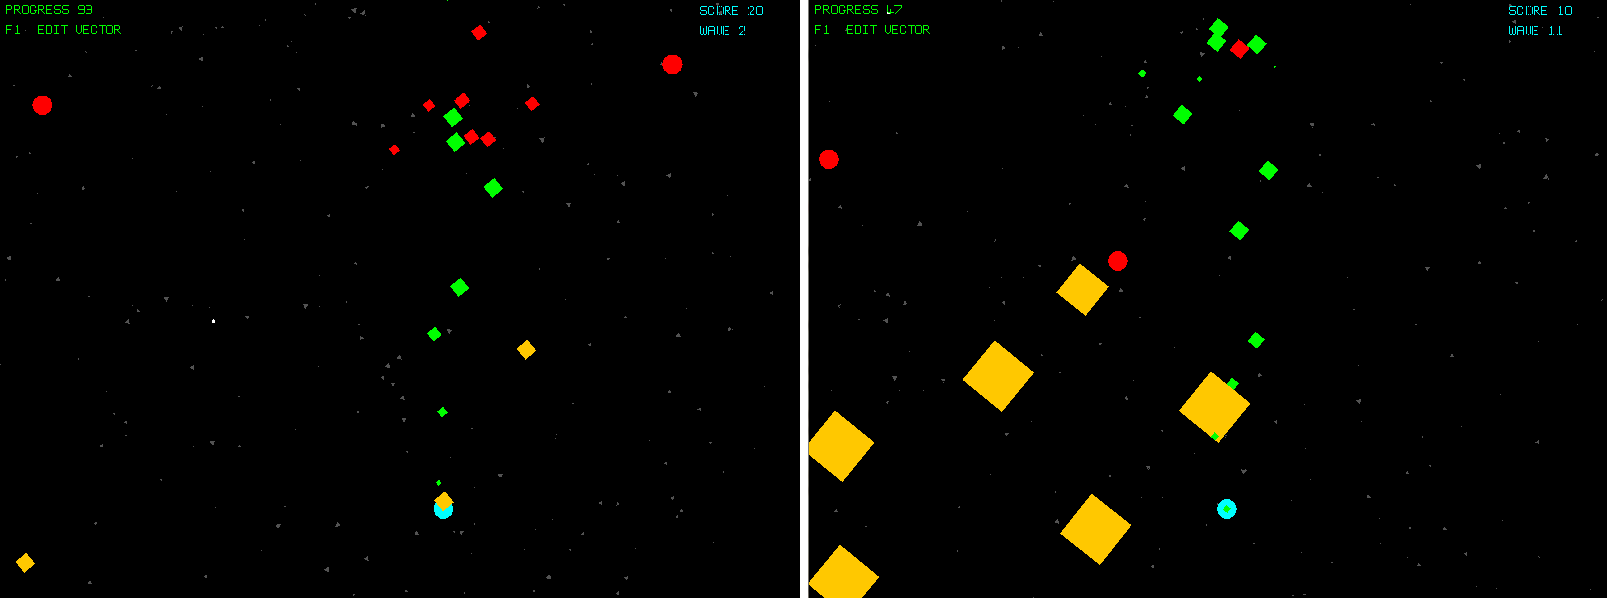
\includegraphics[width=1\linewidth]{./bullethell_sidebyside}
\caption{Experimental game interface illustrating player, enemies, and shots fired by both at two points along adaptation process. Preference learning experiments varied parameters related to player movement; enemy tuning involved the speed, size, and rate of fire of enemy bullets.}
\label{fig:shmup}
\end{figure}

% % SHMUP description: score, params
We test the interactive Bayesian Optimization model in a shoot-'em-up arcade game (Figure \ref{fig:shmup}). 
%The fast, reflex-based gameplay style of the game helps reduce complexities involved in long-term player planning and strategy.
Shoot-'em-up games emphasize reflexes and pattern recognition abilities as a player maneuvers a ship to dodge enemy shots and return fire.
An arcade-style game enables our system to use a series of waves to test game parameter settings and gather feedback from the player, iteratively refining the parameter settings to a given design objective. Further, the action-oriented gameplay reduces the complexities of player long-term planning and strategizing, serving as an ideal starting domain for low-level tuning.
In our game players gain points for defeating enemies and lose points when hit by enemies. Players are encouraged to avoid enemy fire by dodging enemy attacks or destroying enemy ships to (temporarily) reduce the number of incoming attacks.

% % enemy params
During each wave a series of enemies appear that fire bullets at the player. In our experiments, we varied three parameters governing enemy behavior: size of enemy bullets, speed of enemy bullets, and rate that enemies fire bullets. Increasing bullet size requires the player to move more carefully to avoid bullets. Faster bullets require quicker player reflexes to dodge incoming fire. More rapid firing rates increase the volume of incoming fire. Together these three parameters govern how much players must move to dodge enemy attacks, in turn challenging player reflexes. As with controls, getting approximate settings for these parameters is easy, but fine-tuning them for a desired level of difficulty can be challenging. Our performance adaptation experiment had the system set enemy bullet size, speed, and firing rate to minimize the difference between player performance and designer-specified target performance.


% % control params
Player controls are limited to shooting at enemies and moving their ship. 
Ship movement is governed by two controllable parameters: drag and thrust. Drag is the ``friction'' applied to a ship that decelerates the moving ship at a constant rate when it is moving---larger values cause the ship to stop drifting in motion sooner. Thrust is the ``force'' a player movement press applies to accelerate the ship---larger values cause the ship to move more rapidly when the player presses a key to move. 

Combinations of thrust and drag are easy to tune to rough ranges of playability. However, the precise values needed to ensure the player has the appropriate controls are difficult to find as player movement depends on how enemies attack and individual player preferences for control sensitivity (much like mouse movement sensitivity). Our preference-learning experiment had the system set drag and thrust for the player while attempting to maximize player preference for a set of controls.




\section{Interactive Bayesian Optimization}
We use interactive Bayesian Optimization (IBO) to model an iterative game design process informed by playtesting. IBO is itself a form of sequential Bayesian optimization where data points are player feedback gathered in interaction of AI with the user \cite{brochu2010:thesis}.
Sequential Bayesian optimization optimizes a function through iteratively testing a sequence of points, each one selected by some algorithm based on previous points. 
Two functions are involved: (1) the \textit{objective function} that maps inputs to outputs; and (2) the \textit{acquisition function} that maps potential inputs to their value for optimizing the objective function output. 
In our application we employ Gaussian processes (GPs) for the objective function---the game design model from parameters to player behavior---and a modified expected improvement acquisition function---trading exploration of the design space against exploitation of designs known to achieve the design objective.

Gaussian processes are a non-parametric modeling technique able to capture complex non-linear relationships within a data set, automatically adjust model complexity to data, and integrate out parameters without user intervention \cite{rasmussen2006}. Intuitively, non-parametric models allow an infinite number of variables to account for the data before selecting only the subset needed to explain a given set of observations. In practice, this leads to models that automatically become more complex to fit a data set as needed. 
Bayesian formulations of GP regression and classification automatically trade off between model complexity and fit to a data set, avoiding over-fitting and poor generalization problems that occur with other optimization approaches. Bayesian model specifications allow parameters of the model to be integrated out, simplifying their use by requiring less user specification. We employ GPs to leverage the benefits of non-linear mapping from inputs to outputs, automatic complexity adjustment with data collection, and reduced or eliminated parameter specification from users.

Below we describe the standard formulations of GP regression and GP preference learning and then integrate GP models with active learning methods for a full IBO model. We demonstrate how the IBO approach can use existing GP models to automate design tuning and learning a design space model.
Gaussian process regression enables automatic difficulty adjustment by modeling player performance in a game as a non-linear function of game parameters. Gaussian process preference learning enables optimization of game parameters (here controls) to player preferences by modeling player preferences for a set of game parameters as a non-linear function of game parameters that is forced to pairwise choices between alternatives. Active learning uses a GP objective function to identify the next parameter settings to test, guided by a designer-specified acquisition function---here expected improvement---for parameter adjustment. For game performance, designers specify a goal of achieving a given level of in-game performance; for controls, designers specify optimal player preference.

\subsection{Gaussian Process Regression}
Gaussian processes are formally defined as ``a collection of random variables, any finite number of which have a joint Gaussian distribution'' \cite{rasmussen2006}. While allowing an infinite number of variables to be used, any GP model can be computed through a multivariate Gaussian distribution based on the input and output values. Gaussian processes are specified by their mean function ($m(x)$) and covariance function ($k(x,x')$):

$$ f(x) \thicksim GP( m(x), k(x,x') ) $$
Intuitively, GP regression learns a model predicting that similar inputs---according to the covariance function---should yield similar outputs. Different covariance functions define different notions of similarity. In our work we employ the automatic relevancy detection (ARD) version of a squared exponential distance:

$$ k(x,x') = exp\big( -\frac{1}{2} \Sigma_{l=1}^{d} \kappa^{l} (x^{l} - x'^{l})^2 \big) $$
where $\kappa^{l} > 0$ is the ARD parameter for the $l$-th feature of a {d}-dimensional data set, serving to control the contribution of this feature to the model. Automatic relevancy detection allows us to optimize model parameters during the fitting process, automatically scaling input dimensions to minimize the impact of irrelevant aspects of the data. Mathematical properties of the GP mean that an initially zero valued mean function will taken on non-zero values after fitting data, allowing the model to be initialized with zero as the mean value (see \cite{rasmussen2006} for additional details on GP regression). In our case we use such a zero-mean GP.

For our performance regression model we predict player performance (number of times hit) from game parameters controlling enemy attacks (speed and size of bullets along with firing rate). We fit a GP regression model to player data and optimize the covariance function ARD parameters using stochastic gradient descent after each training point received. Since GP regression has a closed-form solution for learning and prediction the primary computational bottleneck is optimizing the ARD parameters (needing 13 seconds for 10 training points on a standard desktop machine).

\subsection{Gaussian Process Preference Learning}
We employ a pairwise preference learning model rather than using preference rating scales due to human biases. Sequential numeric ratings are subject to a cognitive anchoring bias where earlier numeric ratings influence choices on subsequent ratings \cite{tversky1974:biases}. We thus employ a model that generalizes information gained from pairwise rankings to the underlying preference of users for different instances (here game parameter settings). Games can only be played sequentially during comparisons, motivating an approach of pairwise preference ratings comparing each new instance to the previous one.

Gaussian process preference learning models user choices in a two-part model: (1) a GP regression model specifying the underlying  (unobserved) value of a single instance; (2) a probit model of how a choice is generated based on two instances being compared \cite{chu2005}. The GP model allows a flexible specification of how users value a given instance specified in terms of its parameters. The probit model---known in economics as the Thurstone-Mosteller law of comparative judgment---converts a pair of latent values into a comparison judgment according to the function:

$$ P( x_i \succ x_j | f(x_i), f(x_j) = \Phi\bigg( \frac{f(x_j) - f_(x_j)}{\sqrt{2} \sigma_{noise}} \bigg) $$
where $x_i, x_j$ are two instances, $f(x_i)$ is the GP latent value of an instance, $\Phi$ is the cumulative normal distribution, and $\sigma_{noise}$ is the inherent noisiness of comparative judgments. Intuitively, the probit model encodes preference judgments as based on the difference in underlying value of two instances, allowing for noise in preference ratings. 

Due to the non-linear probit model used GP preference learning has no analytic learning model. Instead, we follow work by \cite{chu2005} and use a Laplace approximation to learn the underlying GP model's parameters. We employ a GP with zero mean and the ARD covariance function and optimize its parameters along with the selection of $\sigma_{noise}$ using a grid search over the space of possible parameters. These nested optimization processes are possible using off-the-shelf solvers, requiring 9 seconds for 10 training points. 
We note that optimization may be performed using any-time algorithms (such as DIRECT \cite{jones1993:direct}), allowing optimization of parameters to occur while the player plays a new option. In our experiments we optimize parameter values and force players to wait in order to test the best-case performance of our approach.


\subsection{Active Learning}
Active learning (AL) is an approach to machine learning problems with a large set of unlabeled instances where a computer asks a human to provide information about given instances to learn a model of the instances as a whole \cite{settles2012:al-book}. AL is well suited to our application where the space of game parameterizations is very large and information can only be gained through the expensive process of having a human play and provide feedback about a game instance. Acquisition functions specify how a given AL algorithm weights potential instances to test based on a goal of optimizing the objective function. In our case, the GP regression model seeks to minimize the difference between desired and actual player performance and the GP preference model seeks to find the highest latent value instance.

Many possible acquisition functions exist, varying in how the functions balance the exploration-exploitation trade-off guiding how locally-tethered the search for large objective function values is \cite{settles2012:al-book}. Expected improvement (EI) is an acquisition function that balances the value of unseen instances against the uncertainty regarding their values. EI integrates over all possible results to get an average-case estimate of the result, rather than seeking a best-case (or worst-case) scenario. We employ a modified EI function that incorporates a slack parameter ($\xi \ge 0$) to control the relative weighting of exploration and exploitation goals \cite{lizotte2008}:

% % clean up formatting to fit width
$$ EI(x) = \begin{cases} 
(f(x) - f(x^{+}) - \xi \Phi(Z) + \\ \sigma(x) \phi(Z)) & \mbox{if } \sigma(x) > 0 \\ 
0 & \mbox{if } \sigma(x) = 0 
\end{cases} $$
where $f(x)$ is the function value at $x$, $x^{+}$ is the instance with the current greatest function value, $\sigma{x}$ is the uncertainty in the value of the instance, $\phi(Z)$ is the Gaussian distribution density at $Z$ and $Z$ is defined as:

$$ Z = \begin{cases} 
\frac{f(x) - f(x^{+}) - \xi}{\sigma(x)} & \mbox{if } \sigma(x) > 0 \\ 
0 & \mbox{if } \sigma(x) = 0 
\end{cases} $$
Intuitively, $Z$ is the noise-scaled difference between the test point $x$ and the current best point $x^{+}$, and the expected improvement takes a weighted combination of this gain against the uncertainty of the point. Points that are more uncertain and expected to have higher values are preferred to those with lower values or high values that are highly certain. $\xi$ allows an explicit specification of how heavily to emphasize exploration



\section{Experiment}
% % goal = assess model ability to:
% % % regression = fit player to target behavior
% % % preference = get controls that "suit" player --> Q: how know when "good enough"?
In this section we describe two empirical human studies we conducted. The first study examines the use of GP regression to find and continually adjust game parameter settings to achieve a designer-specified level of performance. The second study examines the use of GP preference modeling to optimize controls to player preferences. We show our approach, compared to random sampling: improves a player model's predictive power with the same sampling budget, does equally well or better at achieving a design objective, and improves the ratio of positive to negative responses to sample points in preference learning. Random sampling is the common standard used to evaluate the efficacy of AL models for improving model fits for a given data budget and is similar to A/B testing approaches that capture large amounts of data before acting on the results \cite{settles2012:al-book}.


\subsection{Methods}
% % conditions test different cases for regression-based adaptation + preference learning
We used 60 \todo{update} sessions of data in both studies. Players logged into the game online and played the game against a series of waves of enemies. Players were assigned in a balanced factorial design to either a control case that sampled random possible game parameter values or a test case that selected parameter values using interactive Bayesian optimization.
%Players were allowed to play up to 5\todo{update}, 30 second-long waves of enemies in a fixed tutorial mode to familiarize themselves with the game. For both studies players completed 15\todo{update} waves of enemies. 
We recorded player performance in terms of number of times the player was hit and all parameter settings for each wave. Player preferences were recorded in a four option forced choice pane, selecting whether the control settings of the current wave compared to the previous wave were: better, worse, no different, or different but of equal quality.
For analysis we examined only results from players who completed at least ten waves and only examine data from those ten waves. Preference responses only used better or worse choices.

In the performance optimization study a GP regression model was fit to predict the difference between the actual number of times the player was hit and a desired designer-specified value. We specified a designer target of players being hit 6 times over the course of a 20 second wave of combat. Between waves the model and covariance function parameters were all optimized and EI used to select the next test point.
Learning had a one wave lag---players were allowed to play a wave while the model was fit on a server machine to all data but the most recent wave. This enabled the game to play continuously without pausing for learning to occur at the cost of a model that was unaware of the most recent test point results.

In the control optimization study a GP preference model was fit to predict the underlying preference players had for different control settings. After each wave players were prompted to indicate whether the most recent wave had better or worse controls than the wave before that. Model fitting used the same timing as above. In this case EI selected an instance to test in comparison to the last tested instance---every comparison was the next point that would be most useful compared to the last level the player completed.



\subsection{Results}



\section{Discussion}
% % recap
% modeling design space --> can visualize or be used by designers
% tailoring --> online adjustment of games to players
% formalization --> support more understanding of AI in design process, rather than just produce assets; link player modeling with procedural content

% % vision: game design cognitive architecture, capturing _process of game design, not just reproducing _product

% % value for optimizing subjective or objective results

% % note: can combine multiple aspects into single acquisition function, but then need additional complexity of learning how to balance objectives if not told directly; e.g. preference + performance

% % enable continuous model improvement

% % future: optimal experimental design (rafferty, chaloner); hcomp for more direct human participation


\section{Acknowledgments}
% Eric Fruchter - or possible co-author

\bibliographystyle{aaai}
\bibliography{lib}

\end{document}
